\documentclass[10pt, a4paper]{article}
% \documentclass[twocolumn]{article}

\usepackage[latin1]{inputenc}
\usepackage{amsmath}
\usepackage{amsfonts}
\usepackage{amssymb}
\usepackage{graphicx}
\usepackage{xcolor}
\usepackage{float}
\usepackage{hyperref}
\usepackage{booktabs}
\usepackage[normalem]{ulem}
\usepackage{cite}

\usepackage{xcolor}
\hypersetup{
    colorlinks,
    linkcolor={red!50!black},
    citecolor={blue!50!black},
    urlcolor={blue!80!black}
}

% Forcequit autonumbering
\pagenumbering{gobble}


%% Multicolumns
\usepackage{multicol}
\setlength{\columnsep}{1cm}


% Margin to left and middle
\usepackage[margin={2cm,1cm}]{geometry}

\usepackage{subcaption}


\title{Immaterialist Fashion - Report}

\author{Mick van Hulst \and Dennis Verheijden \and Roel van der burg \and Brian Westerweel \and Joost Besseling}

\begin{document}
	\maketitle
	
	%% Start multicolumns
	\begin{multicols}{2}
	
	    \section{Introduction}
	    This report describes the results for the second competition of the course Machine Learning in Practice. The source code for this project can be found by going to \href{https://github.com/mickvanhulst/imaterialist_kaggle}{the public Github repository}.
	    \\
	    \\
	    During the project each of the team members were assigned specific tasks. Do take note that our approach can be considered agile as we switched roles constantly and helped each other out where we could:
	    \begin{itemize}
	        \item \textbf{Mick van Hulst:} Batch generator (e.g. probability sampling and class weights), Exploratory data analysis, GCP integration in pipeline, Ensembling, thresholding and report.
	        \item \textbf{Dennis Verheijen:} Implementing networks (InceptionV3 and Xception), maintaining ML pipeline, Training networks 
	        \item \textbf{Roel van der Burg:} BatchGenerator, Exploratory data analysis, implementing ResNet, thresholding and report.
	        \item \textbf{Brian Westerweel:} Implementing custom F1-measure, Object-detection, Report
	        \item \textbf{Joost Besseling:} Object-detection, Ensemble algorithm
	    \end{itemize}
		
		\section{Problem statement}
		We have chosen \href{https://www.kaggle.com/c/imaterialist-challenge-fashion-2018}{the immaterialist fashion challenge} on Kaggle. This challenge consisted of a data set of approximately 1.1 million images which had to be assigned to one or multiple labels. In total there are 228 labels that could be assigned.
		
		\section{Data set}
        The data set that the challenge provides consists of a training, test and validation set, which in turn consist of: 
        \begin{itemize}
            \item 1.014.544 training images;
            \item 228 labels in the training dataset;
            \item 39.706 test images;
            \item 9.897 validation images;
            \item 225 labels in validation set.
        \end{itemize}
        We're interested in the distributions of the data such that we can prepare our models accordingly. Figure \ref{fig:data_dist_train} and \ref{fig:data_dist_val} visualise the distribution of the labels for the training and validation dataset respectively. We observe that the labels aren't evenly distributed, but the distribution between the training and validation dataset seems comparable.
        \begin{figure}[H]
            \centering
            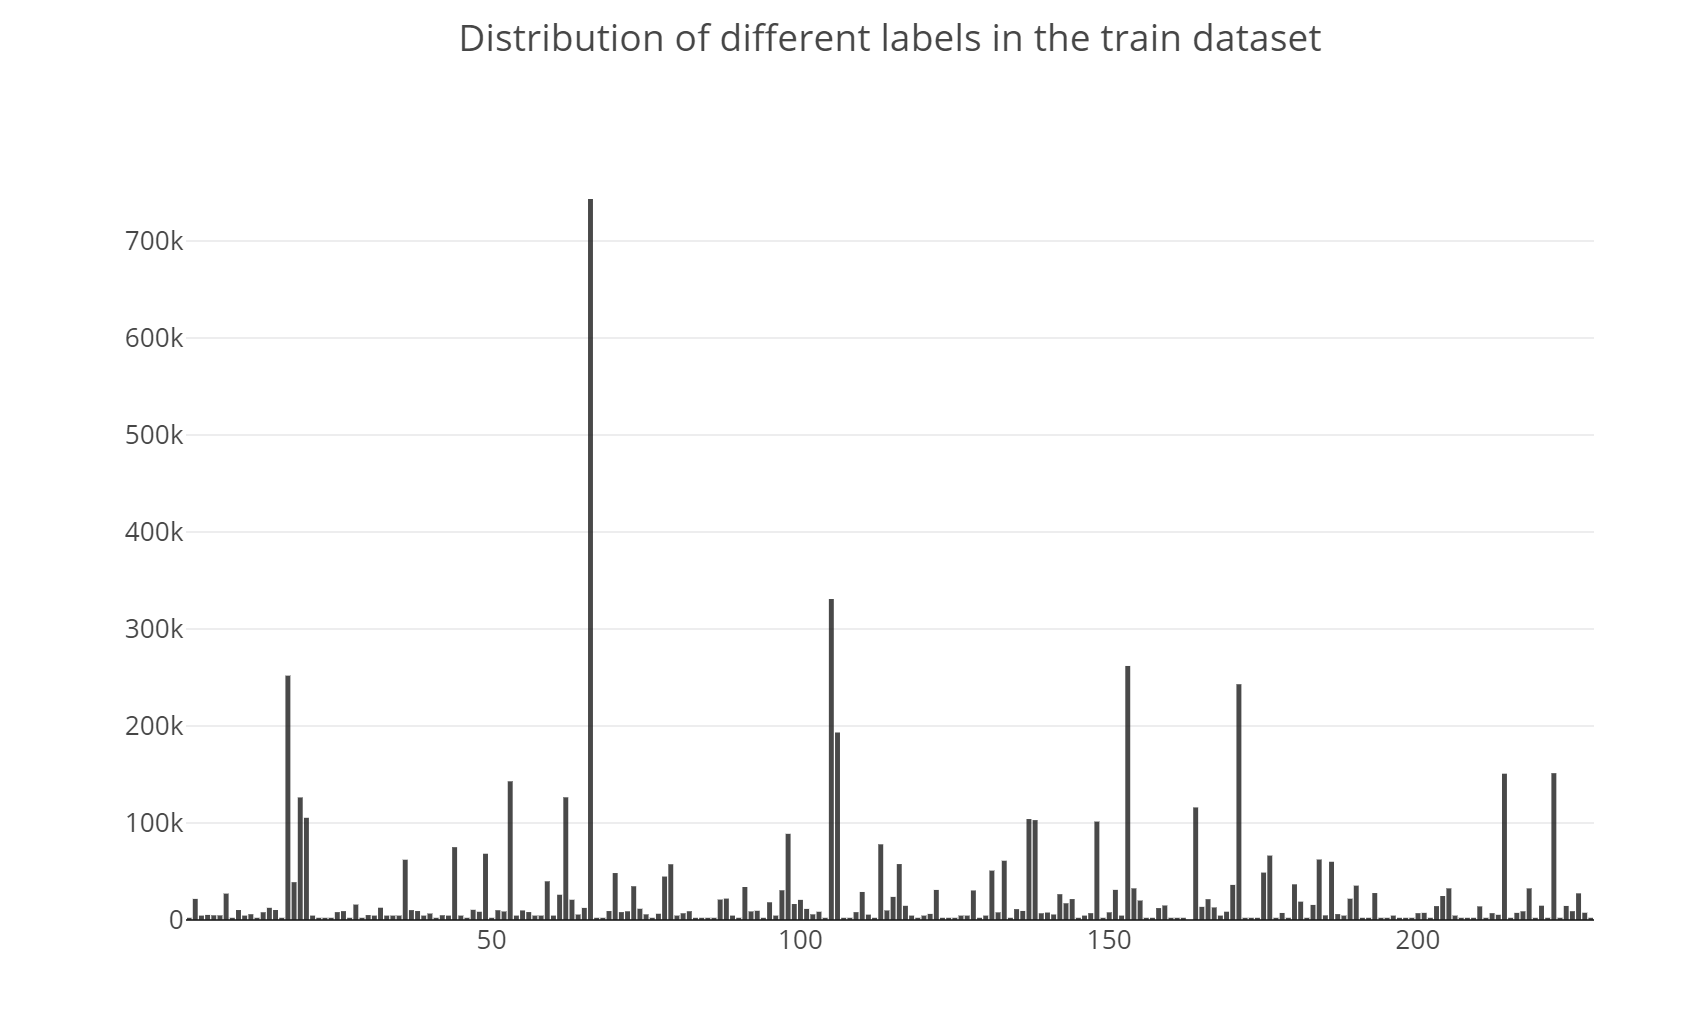
\includegraphics[scale=.4]{img/dist_labels_train.PNG}
            \caption{Data distribution training set}
            \label{fig:data_dist_train}
        \end{figure}
        
        \begin{figure}[H]
            \centering
            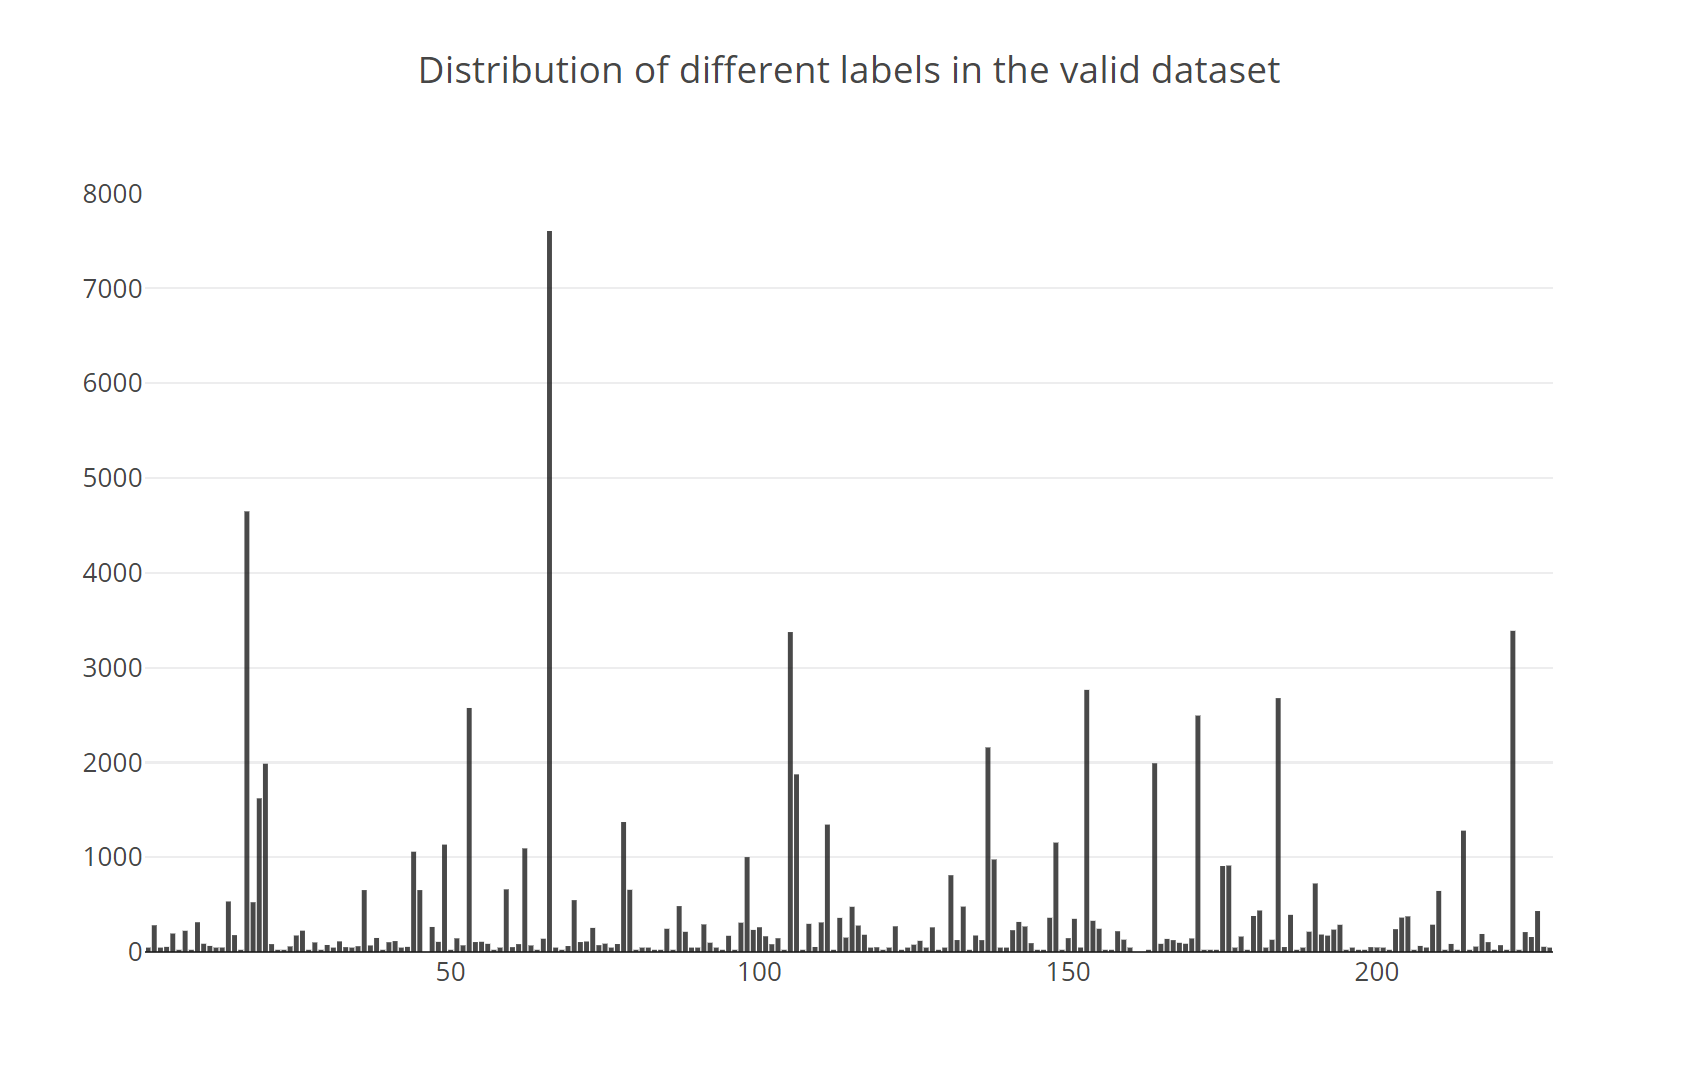
\includegraphics[scale=.4]{img/dist_labels_validation.PNG}
            \caption{Data distribution validation set}
            \label{fig:data_dist_val}
        \end{figure}
        To get a feeling for the dataset we also visualise some images and observe that for some labels there are no clear characteristics that define the corresponding label (see Figure \ref{fig:img_example}). From this observation we conclude that it would be hard for a human to differentiate between the labels without knowing what the labels mean exactly. We believe that there's some structure to the labels, meaning that there might be some tree-like structure that explains the different combinations between the labels, however, this is not something that the challenge provides so we cannot use this to e.g. define weights when classifying. This is something we'll have to define ourselves.
        \begin{figure}[H]
            \centering
            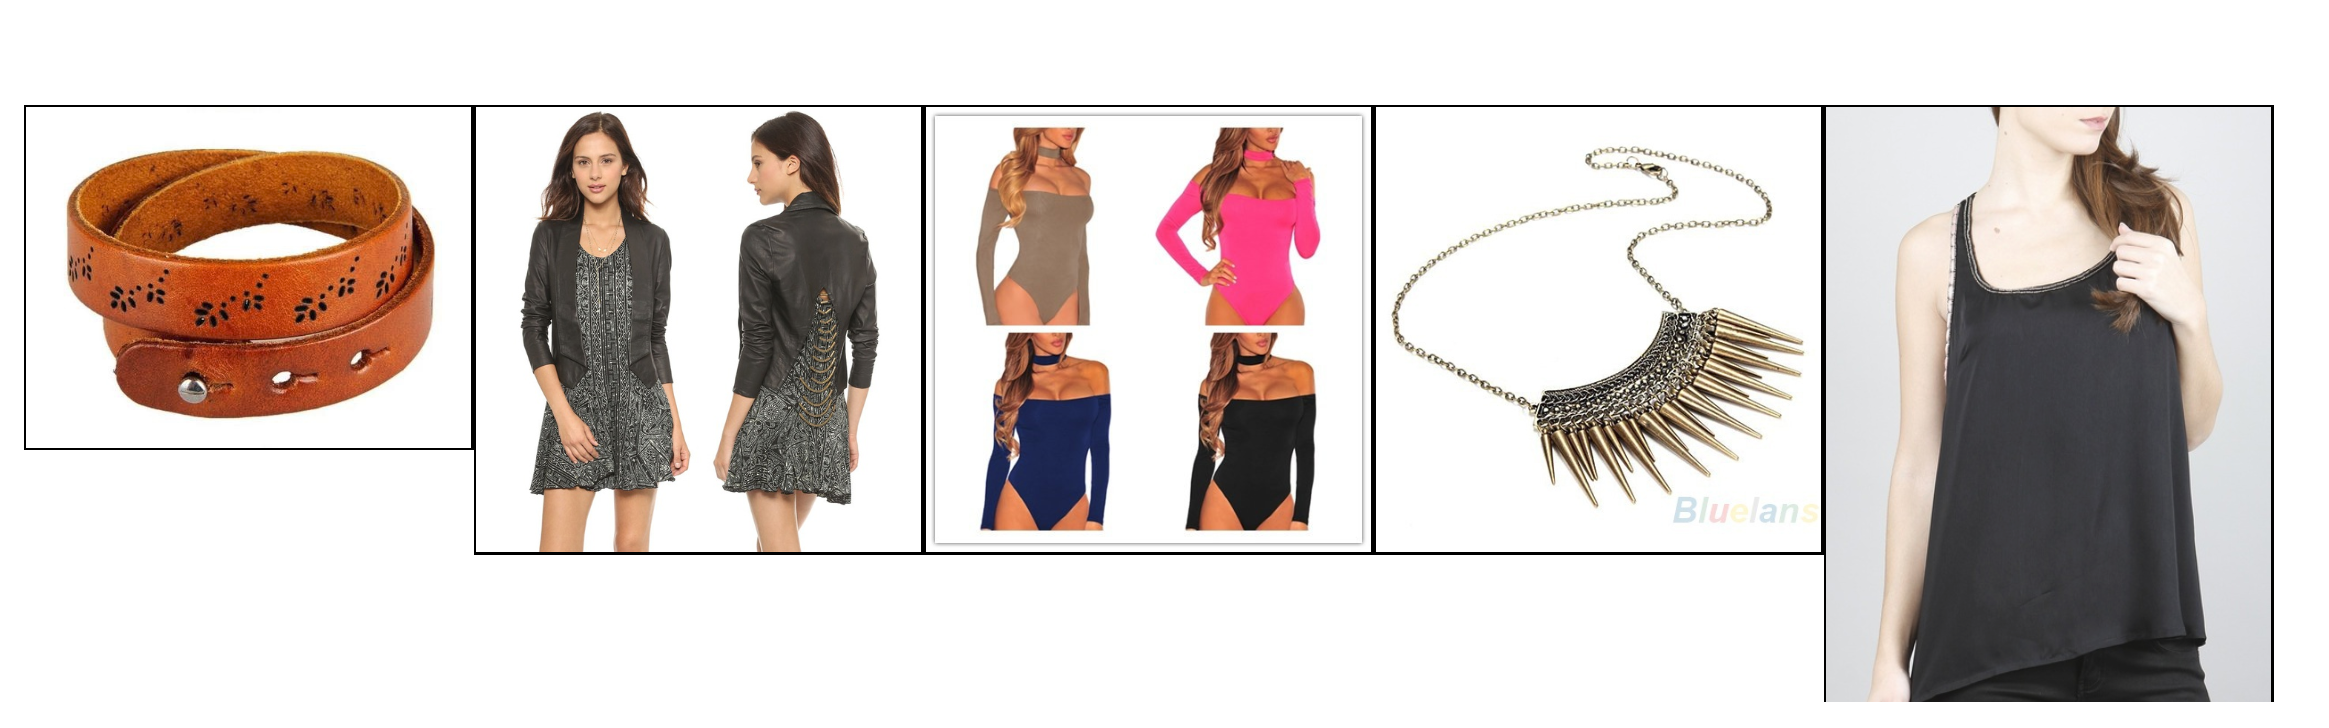
\includegraphics[scale=.2]{img/label_24.jpg}
            \caption{Example image label 24}
            \label{fig:img_example}
        \end{figure}
	
		\section*{Data handling}
		The data for this challenge needed to be cleaned as there existed images which were identical, but had different types of labels. Besides this, the images were also of different sizes, meaning they had to be resized as convolutional neural networks require a static input size. 
		\\
		\\
		It is computationally infeasible to load all the images in the network at once so we developed a batch generator. The batch generator created the possibility to load a set amount of images at a time. To counter the class imbalance we tried probability sampling, however, this didn't render any desirable results as this is a multi-label problem and probability sampling resulted in an identical distribution (i.e. this was most likely due to the top 10 classes occurring for almost every class).
		\\
		\\
		One can observe that the training data set is huge. During training we noticed that generating batches took a long time as we had to continuously download and store the images temporarily. To counter this we uploaded the entire data set to GCP with a 85\% quality to increase the generation of batches and decrease the total file/image size respectively.
		\\
		\\
		The last thing that needs to be noted is that we decided to ignore labels that occurred less than 500 times as we wanted to avoid training the classifiers on labels that didn't occur frequently. We experimented with 5.000 and 500, but noticed that 5.000 ignored too much and thus decided on 500.
		
		\section{Results}
		In contrast to the last project we decided to use pre-trained model for this challenge, instead of fully training the models ourselves. The models used in this project are pre-trained using ImageNet \cite{deng2009imagenet}. ImageNet is a collection of over 100.000 concepts with average 1000 images per concept. Also, ImageNet is often used as a reference data set for setting convolutional neural network benchmarks. For this project MobileNet, InceptionV3, Xception and ResNet50 are chosen because these model individually have a good performance for image classification problems. Therefore, we think that combining the models with ensemble learning methods will yield even better results. Besides the well-known models we created a model based on object detection. In this way we ensure that the data knows all the possible labels it has to predict and the relation between the target data and the labels. By using the pre-trained weights for the different models they are already aware of the high-level abstraction for images. These abstractions have proven to work well on image classification tasks \cite{razavian2014cnn}.
		For fine-tuning the different models the last layers of each models are unfrozen. Unfreezing the last layers make it possible to train them on another data set. These partly unfrozen models are trained on the training data from the challenge.
		\\
		\\
		For the loss of all models binary cross entropy is used, because the model has to output a probability for each label. To measure performance of the models a micro-averaged F1-score is used, because this also is the performance metric used by Kaggle. Hyper parameters are left as they were implemented by Keras.
		\\
		\\
		\textbf{F1-score and early stoppage. Mention something about this here.}

		\subsection{Object detection}
		As we had the suspicion that there was probably some relation between the labels, we thought it would be interesting to try an object detection algorithm. We tried predicting objects for each image using a pretrained ResNet50 \cite{DBLP:journals/corr/HeZRS15}. This network was trained on the open image data set \cite{openimages}. For each image we wanted to use the discovered objects as features for that image and use those images as features to train other neural networks. 
		\\
		\\
		The object detection network detected reasonable objects in some cases, but in the majority of the cases it detected objects such as 'clothing' which are meaningless within the iMaterialist challenge (see Figure \ref{fig:object_dress} and \ref{fig:object_necklace_clothing} for an example). Furthermore, the model took around two minutes to detect objects in an image, meaning that we'd need around two million minutes to apply the model to the entire training set. Due to these reasons, we decided to not pursue this method any further.
		
    	\begin{figure}[H]
          \begin{subfigure}[b]{0.3\columnwidth}
            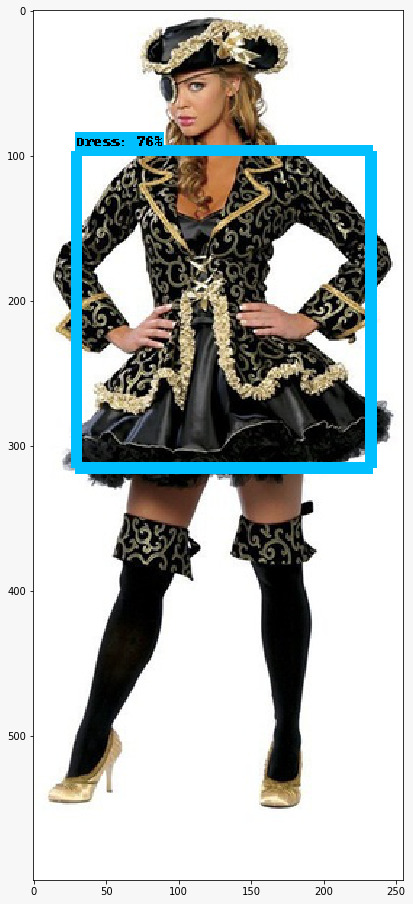
\includegraphics[width=\linewidth]{img/object_detection_img.jpg}
            \caption{Object detection example 'dress'.}
            \label{fig:object_dress}
          \end{subfigure}
          \hfill %%
          \begin{subfigure}[b]{0.4\columnwidth}
            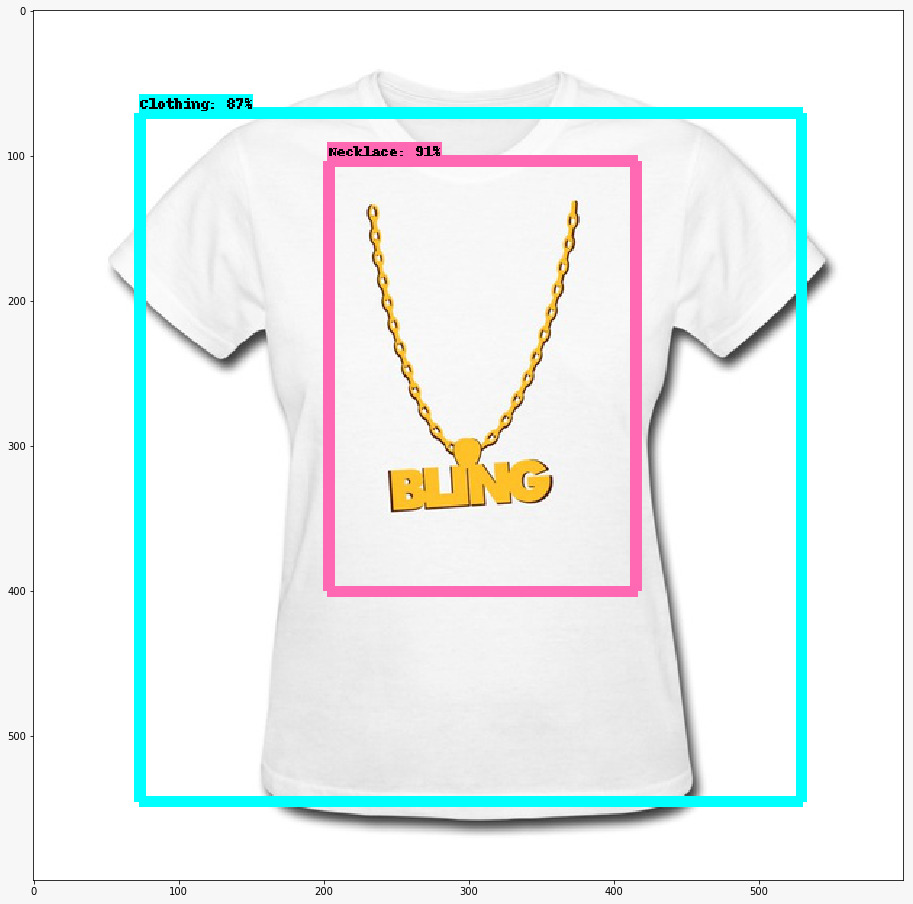
\includegraphics[width=\linewidth]{img/t_shirt_object_detection.jpeg}
            \caption{Object detection example 'necklace' and 'clothing'.}
            \label{fig:object_necklace_clothing}
          \end{subfigure}
        \end{figure}
		
		
		\subsection{ResNet50}
		The ResNet we used is based on Keras' version \cite{DBLP:journals/corr/HeZRS15}, where the last layers were unfrozen and fine-tuned to our target data set. Resnet-50 was a 
		1st place mode for the ILSVRC 2015 classification competition on imagenet.It solves a degregation problem of deeper networks: when network depth increases, accuracy could get saturated. The degradation problem suggest that solver's might have difficulties in approximating identity mappings by multiple nonlinear layers \cite{he2016deep}.
		By dividing the network in residual blocks, it is easier to map these identity mappings by multiple nonlinear layers.
		
		\subsection{MobileNet}
		MobileNet is a convolutional network by (Howard et al, 2017) \cite{howard2017mobilenets}. This network is designed to be ran on mobile devices, which makes it an ideal candidate to do pilot studies with. Which was mainly its usage in this project. It was used to experiment with certain hyperparameters and for testing if the batch generator was working correctly. In this case only the last 5 layers are unfrozen and open for training. MobileNet presents an efficient and powerful deep-learning model by focusing on depthwise separable convolutions. 
		
		\subsection{InceptionV3}
		The inceptionV3 \cite{DBLP:journals/corr/SzegedyVISW15} is a convolutional neural network developed by Google. Inception differs from other conventional neural networks in the way that their lower-level layers are built.
		
		Usually a decision has to be made for each convolutions layer with respect to its layers (i.e 5x5, 3x3 or Max-Pooling). Inception refuses to make the choice for one layer above the other and decided to do everything within one layer. This architecture makes the network very time expensive to train because it is basically brute-forcing the different options that are available.
		
		The InceptionV3 network was trained three times. The first network we trained was an Inception v3 network which we trained on the entire data set. The second and the third network where used to counter the highly imbalanced data set (see Figure \ref{fig:data_dist} for distribution classes). The second classifier is only trained on the labels that occur at least 100.000 times. The third classifier is trained on labels that occur less than 100.000. These two classifiers were combined as by simply adding their predictions. 

		\subsection{Xception}
		The XCeption network is a network proposed by Chollet in 2016 building on the already existing inceptionV3 networks \cite{chollet2016xception}. 
		It changed the inception modules to depthwise separable convolutions 
		This network was trained once and trained on the entire data set.
		
		\subsection{Ensembling}
		After our previous project, one of our takeaways was to apply ensembling during this project. Ensembling is used to combine several models and thus combine their respective strengths. For our ensembling process we combined the aforementioned InceptionV3 and Xception networks. We ensembled the networks after training the models and were ensembled using the following methods:
		\begin{itemize}
		    \item \textbf{Mean:} Takes the mean of all classifier's results.
		    \item \textbf{Harmonic mean:} Is a special kind of mean which was applied as several other students mentioned that it gave them good results in previous competitions. 
		    \item \textbf{Particle Swarm Optimization:} Using PSO (Particle Swarm Optimization) we were able to find weights which maximized the F1-score given the validation set. This means that we assume that the weights which maximised the validation results would also maximise the results of the test data set. 
		\end{itemize}

		\subsection{Thresholding}
		To submit to Kaggle we had to threshold our results. After using a standard threshold of 0.5 we also decided to try custom thresholding for each label. We tried finding thresholds for each label by trying several thresholds and measuring which threshold would increase the F1-score.
		\\
		\\
		After thresholding we got the following results for each classifier and/or ensemble respectively:
		\\
		\\
		\textbf{ADD ALL RESULTS HERE.}
		\\
		\\
        We can see that the results of the PSO algorithm are the most convincing. If we look at the weights that are generated by this strategy, we can see that the combined classifier is relatively important. This validates our idea that we could counteract the imbalance by training two separate classifiers.

		\begin{table*}[t]
			\centering
			\begin{tabular}{l|c|c}
				\toprule
				\textbf{Method} & \textbf{F1} & \textbf{\#params (Million)}\\
				\midrule
				MobileNet &  & 3.46M \\
				InceptionV3\_small &  & 22.3M\\
				XceptionV3\_small &  & 21.3M\\
				ResNet\_small &  & 26M\\
				Xception\_large &  & TBA\\
				\midrule
				\textbf{Ensemble} & & \\
				\bottomrule
			\end{tabular}
			\caption{Summary of the achieved results, per model and with their corresponding F1 on Kaggle.}
			\label{table:summary_results}
		\end{table*}

		\section{Conclusion}
		\subsection{Google Cloud platform (GCP}
		Many of the implemented models were used (after testing) on the Google cloud platform for final training. Including the InceptionV3 and Xception networks, during the final weeks of the project. Together with the  entire dataset that was already uploaded on the GCP-framework we could adjust our batch generator to directly load the the images from disk instead of the downloading we had been doing until then. Unfortunately GCP prove to be very slow during training time and after 24+ hours of training still did not have processed the one-million plus-sized dataset.
		
		\subsection{Simplicity versus over engineering}
		During the start of the second half of the project we enthusiastically started with discussing several convolution networks, an extensive training pipeline, (weighted) probability sampling, per-class thresholding, potential object recognition for extra features and ensembling methods. Many of these methods did prove to be beneficial. For example per-class thresholding and ensembling did (significantly) improve our results. However, the object recognizition seemed to be an avenue worth exploring but we had to conclude proper pre-trained models for our tasks were not available nor did we have the time to label and train our own network. 
		
		\subsection{Stick with the basics initially}
        There's a trade-off between wanting to learn complex things and achieving desired results. The extra merit from fine tuning, or using different models usually pales in comparison with the basic model that is simply trained longer and has seen more of the data. The best models in our ensembling method for example did not need probability sampling. This does not mean complex methods are always inferior to simple ones. Though it did learn us to first stick with a strong simple baseline model, to have as a checkpoint for later. 
        
        % Having proper SSD memory space for the whole dataset and computing power locally could perhaps given us this insight earlier, instead of relying solely on the GCP. 



	    \section{Who did what}
	    (5) Who did What. In this section you describe the contributions of the individual team members during all the course.


	\bibliographystyle{unsrt}
	\bibliography{bib}
	\end{multicols}
	
\end{document}